\section{Theorie} 
\label{sec:Theorie}

In diesem Kapitel werden die theoretischen Hintergründe dieses Versuches erläutert. Dabei wird insbesondere auf die in der Durchführung verwendeten Schaltungen eingegangen.

\subsection{Operationsverstärker}\label{thopv}

Ein Operationsverstärker, oftmals mit OPV abgekürzt, ist ein Schaltbauteil und zählt zu den Differenzverstärkern.
Das heisst die Differenz zweier Eingangsspannungen $U_+$, $U_-$ wird um einen Faktor verstärkt, welcher idealerweise den $\infty$ beträgt.
Ein OPV besitzt acht Anschlüsse, sogenannte Pins, wovon nur sieben einen tatsächlichen Nutzen haben. 
Die wichtigsten Anschlüsse sind die der beiden Eingangsspannungen, wovon eine invertiert wird, der Anschluss für das Ausgangssignal und zwei Anschlüsse für Versorgungsspannungen.
In \autoref{fig:LM741} ist eine Zuordnung der pins und der genannten Anschlüsse am Beispiel des Operationsverstärkers LM741 zu sehen.\footnote{Bild dem Datatasheet entnommen: https://www.ti.com/product/LM741} 
Zur Orientierung des OPVs dient eine Mulde im Bauteil. 
\begin{figure}
    \centering
    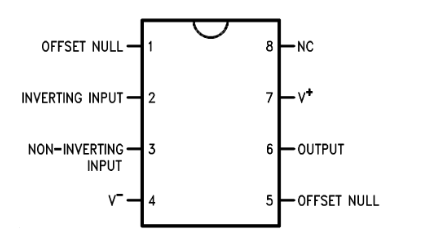
\includegraphics[width=1\textwidth]{content/grafiken/LM741.png}
    \caption{Die 8 pins des LM741 Operationsverstärkers}
    \label{fig:LM741}
\end{figure}
Die Versorgungsspannungen bedingen das Maximum und Minimum der Ausgangsspannung und sind hier symmetrisch um den Nullpunkt angelegt. 
Der maximale Wert U_{a,\text{max}} der Ausgangsspannung $U_a$ ist jedoch endlich und genügt der Bedingung:
\begin{equation} 
|U{a,\text{max}}| < U{V} 
\end{equation} 
Mit |$U_{V+}$| = |$U_{V-}$| = $U_V$ als dem Betrag der Versorgungsspannung.\\

In Schaltungen wird der OPV fast ausschließlich mit Rückkopplung betrieben.
Ist dies als Gegenkopplung realisiert, sind zwei bedeutende Eigenschaften des OPVs als goldene Regeln zusammengefasst.\\
1. Goldene Regel\\
\begin{equation} 
U_+ = U_- 
\end{equation} 
Die Spannungen an den Eingängen sind identisch und somit ist deren Differenz Null.\\
2. Goldene Regel\\
\begin{equation}
I_+ = I_- = 0\,\text{V}
\end{equation} 
Es fließt kein Strom in den Operationsverstärker.




\subsection{Invertierender Linearverstärker}\label{thlinearv}

Ein invertierender Linearverstärker lässt sich mittels eines Operationsverstärkers realisieren, indem das Ausgangssignal auf den invertierenden Eingang des OPV rückgekoppelt wird.
Dazu wird eine Schaltung wie sie in \autoref{fig:SPlinearverstaerker} zu sehen ist verwendet.
Da es sich bei der Rückkopplung um eine Gegenkopplung handelt, dürfen die goldenen Regeln verwendet werden.
Aus der ersten ergibt sich, dass die Spannung am Knotenpunkt zwischen $R_1$ und $R_2$ identisch sein muss. Dieser befindet sich somit virtuell auf Masse.
Die zweite goldene Regel fordert, dass der Strom, der durch $R_1$ fließt, derselbe ist wie der Strom, der durch $R_2$ fließt unter Beachtung der Wahl der Stromflussrichtung.
Daraus ergibt sich folgender Zusammenhang zwischen angelegter Spannung $U_e$ und Ausgangsspannugn $U_a$:
\begin{equation} 
U_a = -\frac{R_2}{R_1}U_e 
\end{equation} 
Das Eingangssignal wird um den endlichen Faktor
\begin{equation} 
V = -\frac{R_2}{R_1}
\end{equation}\label{eq:thverstarkung}
verstärkt. Der Verstärkungsfaktor V hängt theoretisch nur von der Wahl der Widerstände ab.
Praktisch ergibt sich jedoch ein Zusammenhang mit der Frequenz des Eingangssignals, wodurch der Operationsverstärker eine endliche Bandbreite besitzt.
Es zeigt sich, dass die Bandbreite B des OPVs mit dessen Verstärkungsfaktor V folgendermaßen zusammenhängt:
\begin{equation} 
B \cdot V = \text{constant}
\end{equation}



\subsection{Umkehrintegrator und Invertierender Differenzierer}


Durch Aufbau einer Schaltung, wie sie in \autoref{fig:SPumkehrintegrator} zu sehen ist, lässt sich der Operationsverstärker nutzen, um einen Integrator zu realisieren.
Dieser wechselt jedoch auch das Vorzeichen des Eingangssignals und wird somit Umkehrintegrator genannt.
Anstelle eines Widerstandes wird hier ein Kondensator C zur Rückkopplung auf den invertierenden Eingang des OPVs genutzt.
Für den Strom, der durch diesen Kondensator fließt, gilt folgender Zusammenhang:
\begin{equation} 
I_C = C\frac{dU_a}{dt}
\end{equation} 

Die goldenen Regeln werden analog zu \autoref{thlinearv} verwendet. Zur Auflösung der sich ergebenden Gleichung nach $U_a$ wird über die Zeit integriert. Es ergibt sich:
\begin{equation} 
U_a = -\frac{1}{RC} \int U_e \,dt
\end{equation} 

Das Ausgangssignal ist folglich proportional zum zeitlichen Integral über das Eingangssignal.\\
Durch Austausch des Widerstandes mit dem Kondensator wie es in Schaltung \autoref{fig:SPumkehrdifferenzierer} zu sehen ist und analoge Rechnung zu \autoref{thlinearv} ergibt sich dagegen der folgende Zusammenhang:
\begin{equation} 
U_a = -RC \frac{dU_e}{dt}
\end{equation} 
Das Ausgangssignal ist in diesem Fall proportional zur Ableitung des Eingangssignal nach der Zeit.\\



\subsection{Nicht-invertierender Schmitt-Trigger}

Die Schaltung in \autoref{fig:SPschmitttrigger} wird als sogenannter nicht-invertierender Schmitt-Trigger bezeichnet. 
Durch Rückkopplung des Ausgangssignals auf den nicht-invertierenden Eingang des Operationsverstärkers ergibt sich ein Schwellwertschalter.
Wird die Eingangsspannung gegen die Ausgangsspannung aufgetragen ergibt sich als sogenannte Übertragungskennlinie eine Spannungshysterese wie sie in \autoref{fig:thschmitt} zu sehen ist.\footnote{Bild aus: https://www.elektronik-kompendium.de/sites/bau/0209241.htm} 
\begin{figure}
    \centering
    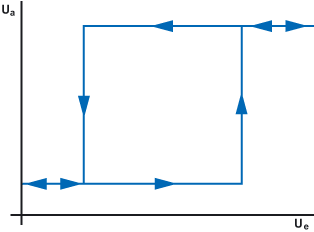
\includegraphics[width=1\textwidth]{content/grafiken/Schmitthysterese.png}
    \caption{Hysterese des nicht-invertierenden Schmitt-Triggers}
    \label{fig:thschmitt}
\end{figure}
Zu erkennen ist, dass das Ausgangssignal für bestimmte Eingangsspannungen sich schlagartig ändert. Diese Kipppunkte lassen sich berechnen zu:
\begin{equation} 
U_{1,2} = \pm \frac{R_1}{R_2} U_V
\end{equation}\label{eq:kipppunkt}
wobei $U_V$ den in \autoref{thopv} beschriebenen Betrag der Versorgungsspannung bezeichnet.





